% This document discusses the benchmarking data. Analysis of what the data means, how it can be interpreted, anything that was unusual or abnormal about the data based on technical review.

\chapter{Results}

\section{Benchmarking}

\subsection{Medium Size File Benchmarking}

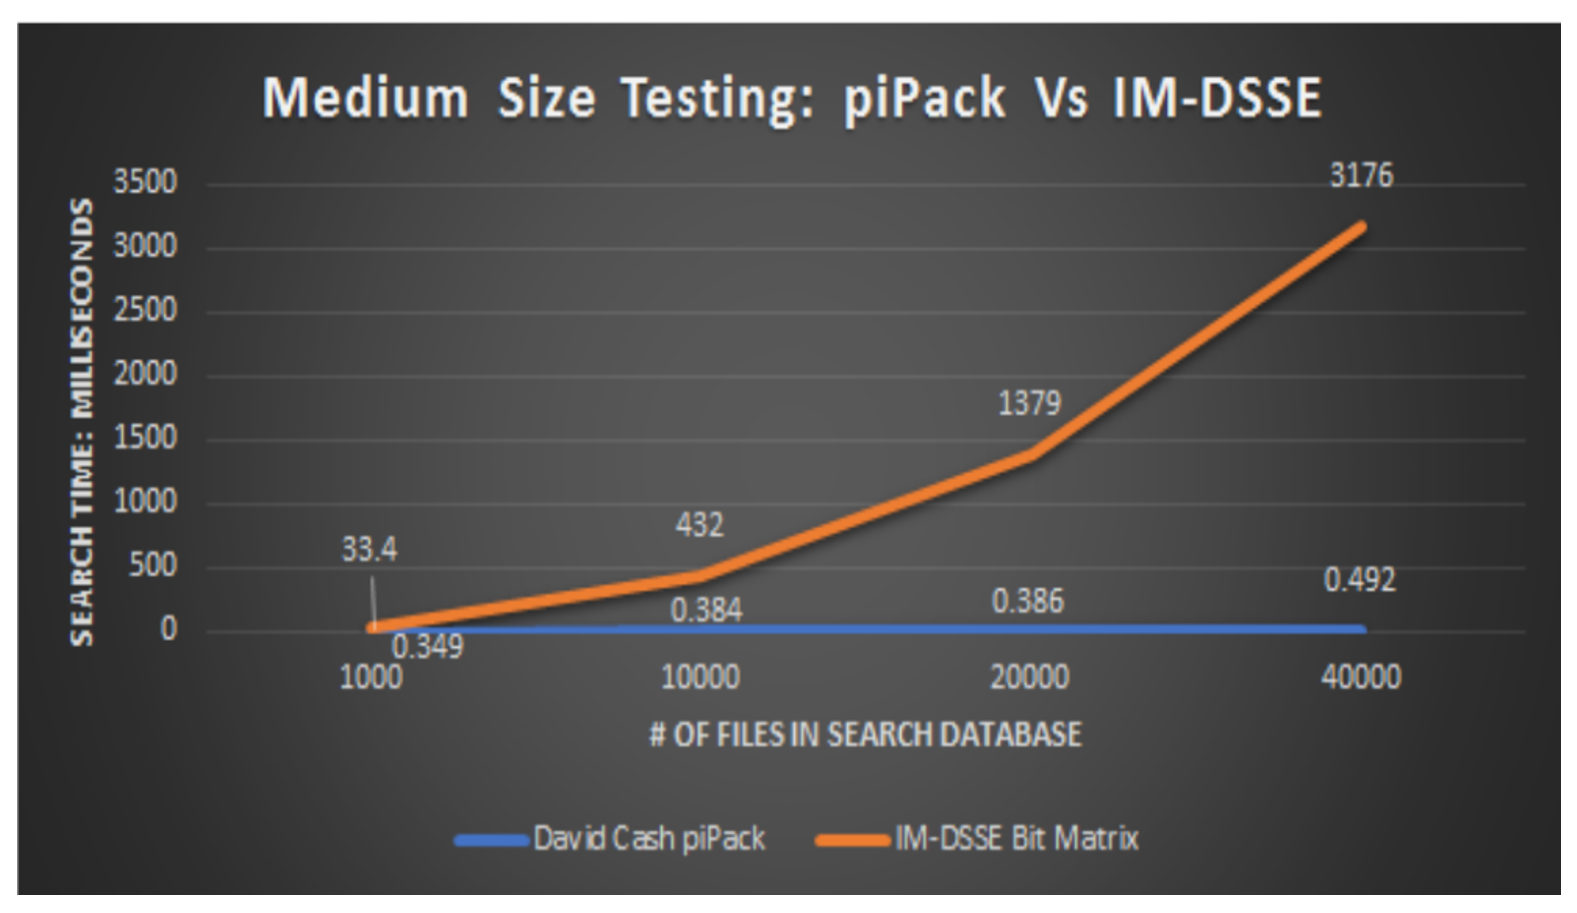
\includegraphics[width=0.8\textwidth]{Charts/medium_size.eps}

The medium size file benchmarking compares the results of IM-DSSE, David Cash Basic and David Cash piPack optimizations to compare the runtime speed of a search call to a database of 1000-40,000 files. Total number of keywords range up to 250,000. As we can see it is very clear that both version of David Cash scheme vastly outperform that of the IM-DSSE Bit Matrix. This makes sense, as we observe that the time complexity for IM-DSSE is $\mathcal{O} (n^2)$ where the search complexity of David Cash is closer to that of $\mathcal{O} (\log n)$. As file sizes increase the runspeed for IM-DSSE is substantially slower than David Cash. We will compare the basic to the optimization of piPack of David Cash in a later graph but we can clearly see here that David Cash has a vastly superior search speed, especially on larger data sets.

\subsection{IM-DSSE Bit Matrix Build time}

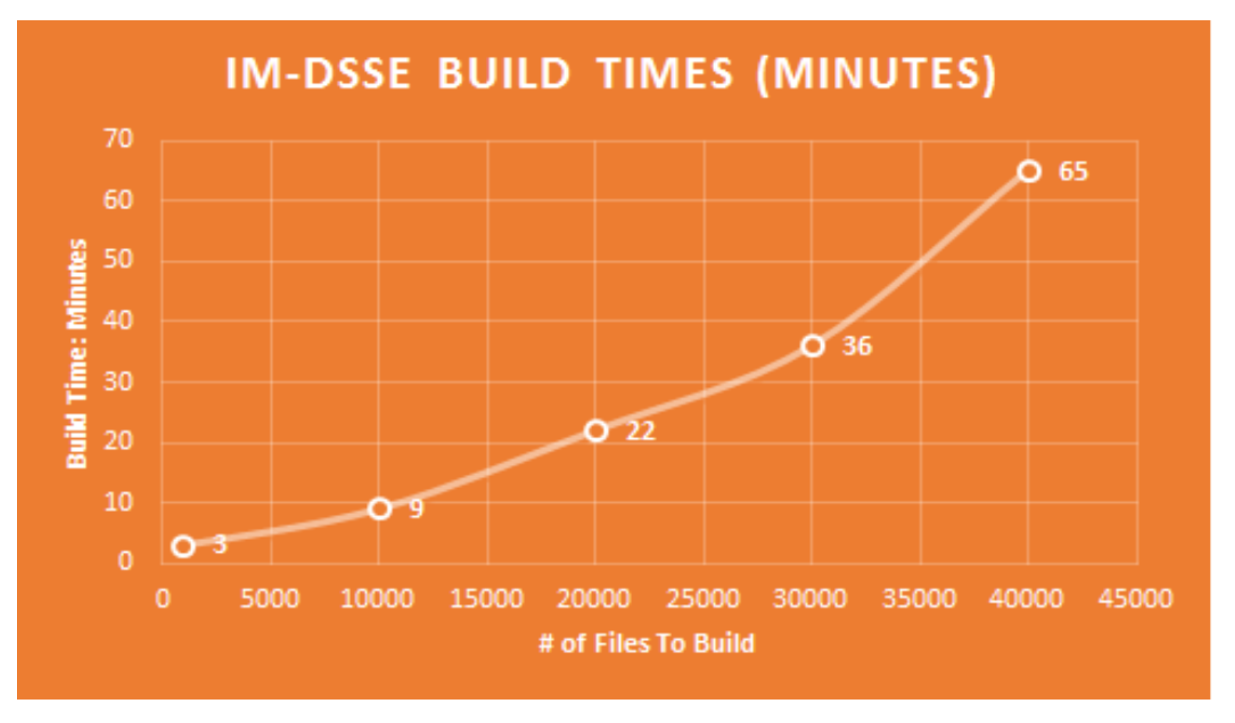
\includegraphics[width=1\textwidth]{Charts/time.eps}

The build time of the IM-DSSE Bit matrix scheme is also $\mathcal{O}(n^2)$ as it needs to create a key file pair with every single file and keyword found in the dataset. This takes a long time, and as a result our testing showed that the quadratic graph confirms that build speed. We did not graph it here but we also averaged out a build time, on the largest dataset of 40,000 files, to be around 2-3 minutes; thus vastly outperforming IM-DSSE at over an hour in build time.

\subsection{Small Data Single file benchmarking}

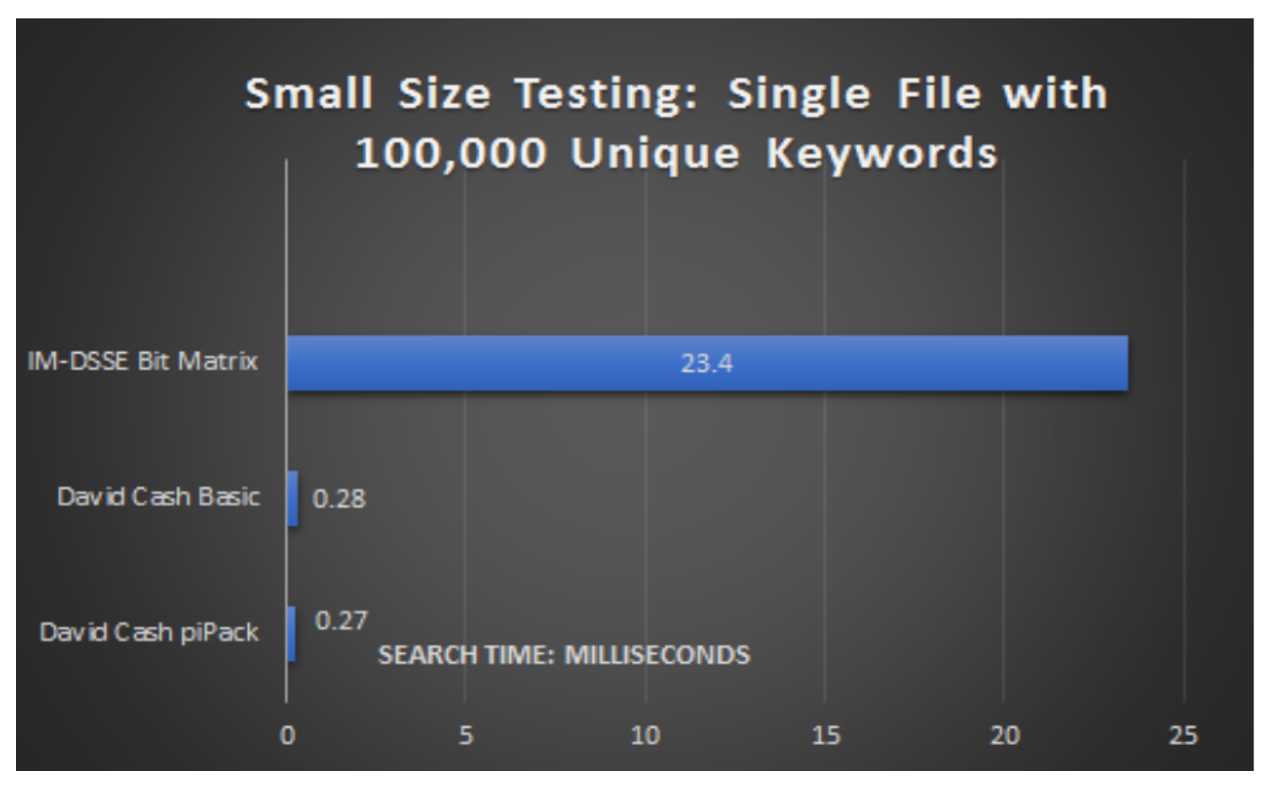
\includegraphics[width=.8\textwidth]{Charts/small.eps}

Similar to the large data set we also see that IM-DSSE is outperformed by David Cash substantially. The overhead of creating this key-file 2d matrix pair is simply much more expensive than the algorithm used by David Cash. The optimization between piPack and Basic is unsubstantial here as we are only working on a single file.

\subsection{DSSE Basic vs DSSE piPack Optimization Graph}

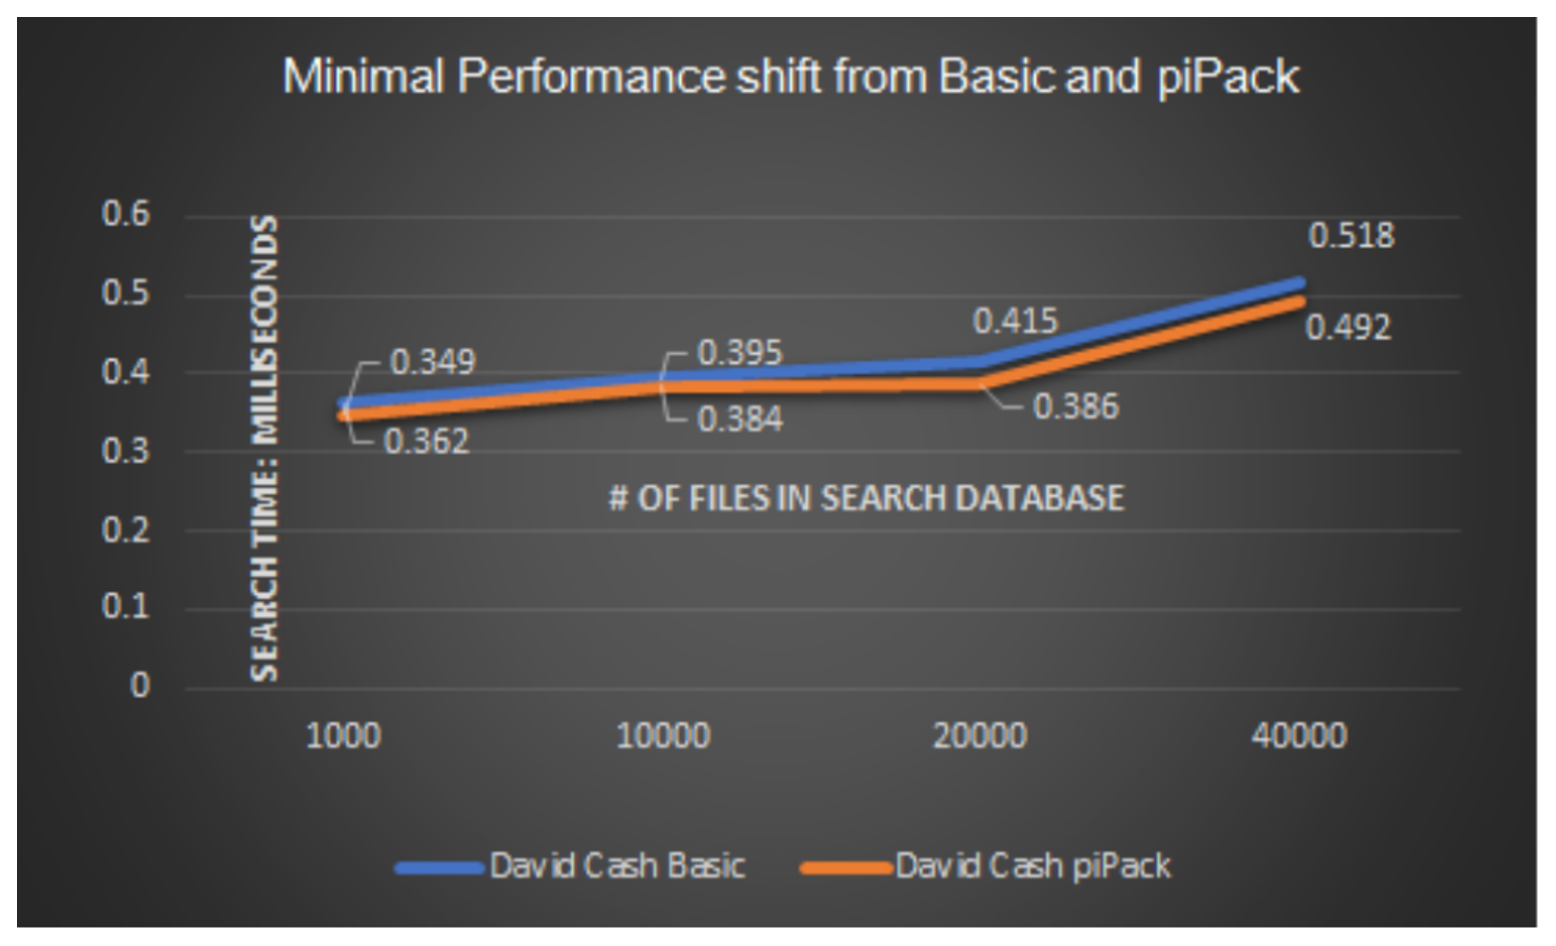
\includegraphics[width=1\textwidth]{Charts/Basic_Vs_piPack.eps}

From our results we believe that this graph is the most interesting to talk about. It is clear that there is a slight optimization between the piPack scheme over the basic. However it was not as large as we were expecting. We believe this is because the piPack scheme would better optimize disk access and data storage retrieval. However, for our testing purposes all the data is stored locally, therefore is on ram. Thus the piPack scheme does not provide much of a benefit.

\subsection{Encrypted Size Comparison DSSE Basic VS IM-DSSE}
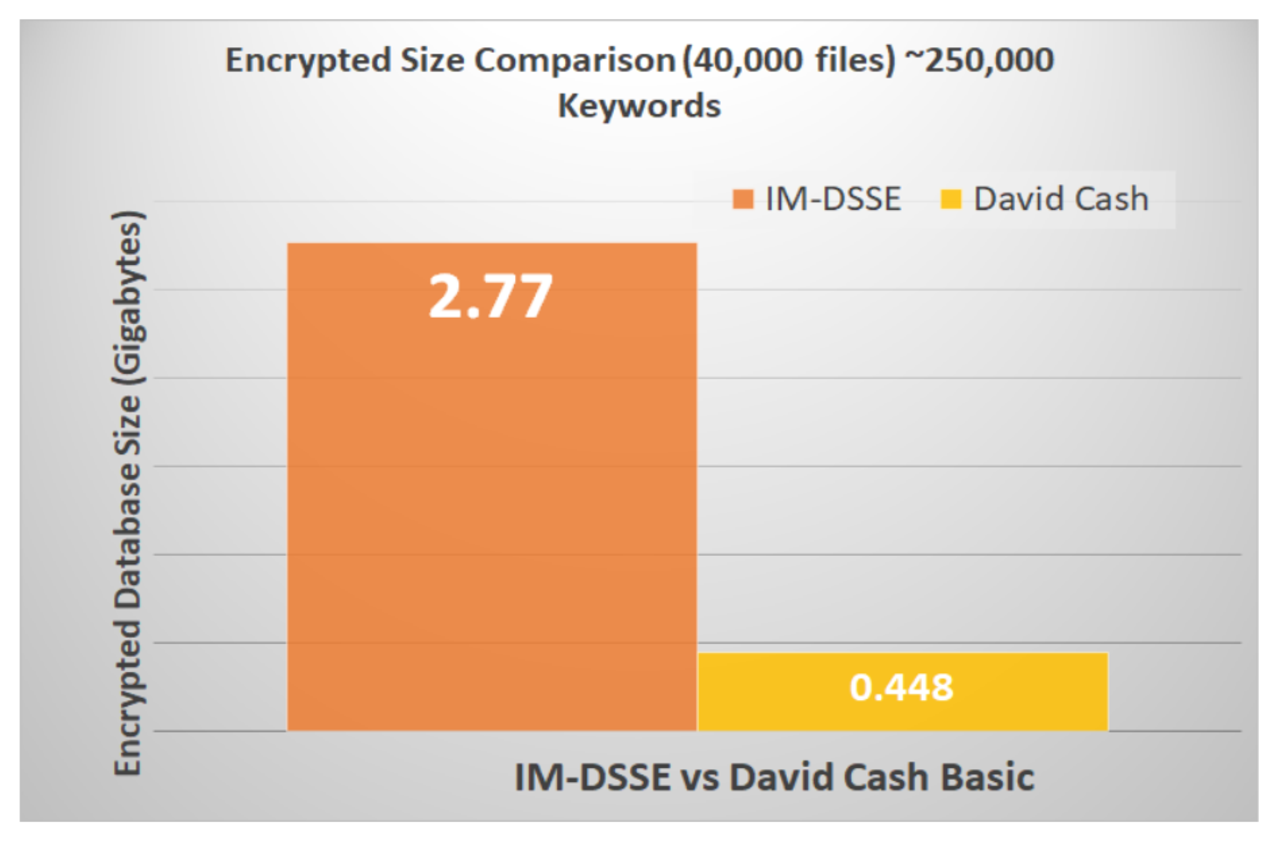
\includegraphics[width=.8\textwidth]{Charts/encrypt.eps}

The encrypted size comparison shows just how much larger the Encrypted Index is that is being searched through between cash and IM-DSSE. In addition to having a slower search time IM-DSSE indirectly composes its own larger dataset to search through because of its implementation of key-file pairs. Thus the size of the datasets are different. I expect this size to become even more drastic were we to test on a large database set such as the Wikipedia text data set.

